\documentclass[12pt,a4paper, russian]{extarticle}
\usepackage[utf8]{inputenc}
\usepackage[T2A]{fontenc}
\usepackage{multirow}
\usepackage{longtable}
\usepackage{amsmath}
\usepackage{amssymb}
\usepackage{graphicx}
\usepackage{newtxmath}
\usepackage{array}
\usepackage[unicode, pdftex]{hyperref}
\usepackage{indentfirst}
\usepackage{longtable,array,colortbl, tabularx, tabulary}
\usepackage{floatrow,floatflt}
\usepackage[tableposition=top, font=normal, justification=centerlast]{caption}
\DeclareCaptionLabelFormat{gostfigure}{Рис. #2}
\DeclareCaptionLabelFormat{gosttable}{Табл. #2}
\DeclareCaptionLabelSeparator{gost}{.~}
\captionsetup[figure]{labelformat=gostfigure, labelsep=gost}

\captionsetup[table]{labelformat=gosttable, labelsep=gost, position=top}
\usepackage{float}
\floatstyle{plaintop}
\restylefloat{table}

\tolerance=500
\emergencystretch=3em
\hfuzz=3pt


\usepackage[english,main=russian]{babel}
\usepackage{titling}
\usepackage{setspace}


\usepackage[a4paper, left=3cm, right=1cm, top=2cm, bottom=2cm]{geometry}
\usepackage{tocloft}
\usepackage{xurl}
\usepackage{ragged2e}
\bibliographystyle{gost-numeric.bbx}
\usepackage{tabularx}
\usepackage[nottoc,numbib]{tocbibind}
\usepackage[
backend=biber, 
sorting=none,
bibstyle=gost-numeric,
citestyle=gost-numeric,
babel=other 
]{biblatex}

\begin{document}
\begin{center}
    \section*{Анализ упаковочных свойств молекул кристаллов кубической сингонии}
\end{center}

Всего проанализированно 889 молекул в 567 структурах, удовлетворяюищх следующим условиям:
\begin{itemize}
\item симметрия структуры описывается пространственной группой кубической сингонии
\item структура в записи не является полимером
\item структура в записи не является разупорядоченной
\end{itemize}

\begin{figure}[H]
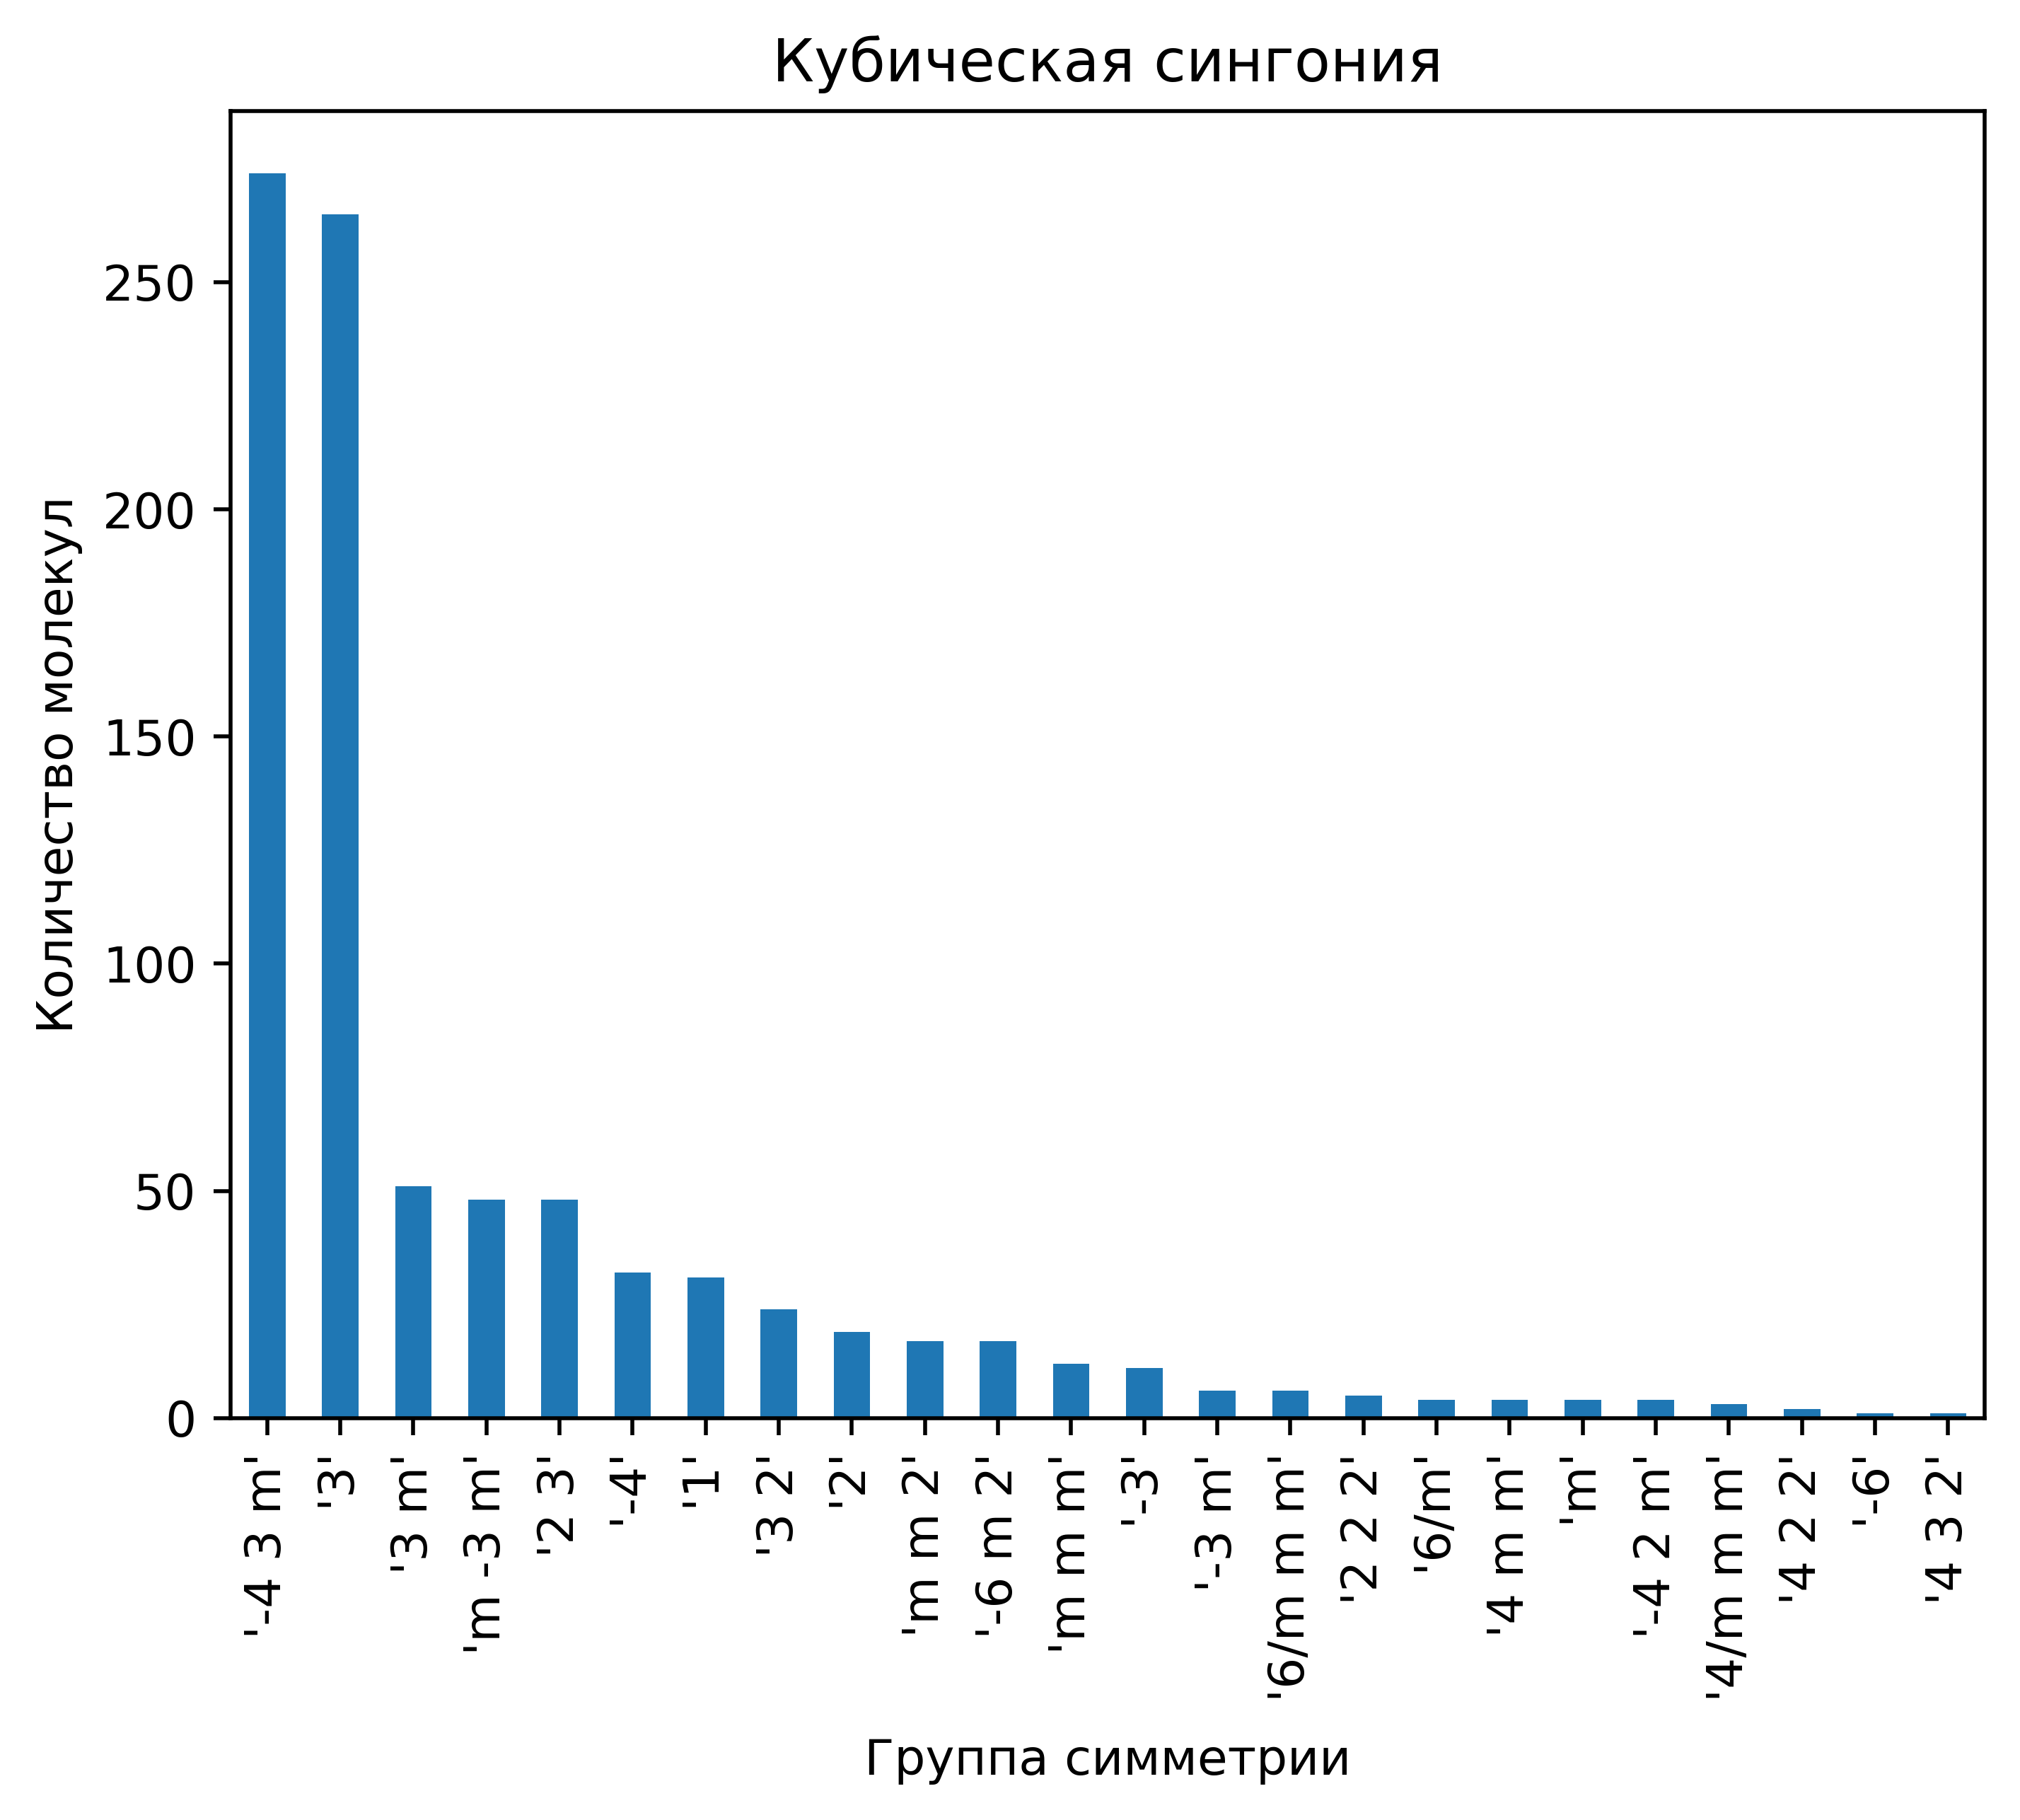
\includegraphics[scale=0.8]{plots_sym/cubic_syngony.png}
\caption{Распределение точечных групп симметрии молекул в кристаллах кубической сингонии}
\end{figure}

\begin{table}[H]
\centering
\begin{tabular}{c|c}
Симметрия молекулы & Кол-во молекул \\
\hline
 '-4 3 m' & 274 \\
 '3' & 265 \\
 '3 m' & 51 \\
 'm -3 m' & 48 \\
 '2 3' & 48 \\
 '-4' & 32 \\
 '1' & 31 \\
 '3 2' & 24 \\
 '2' & 19 \\
 'm m 2' & 17 \\
 '-6 m 2' & 17 \\
 'm m m' & 12 \\
 '-3' & 11 \\
 '-3 m' & 6 \\
 '6/m m m' & 6 \\
 '2 2 2' & 5 \\
 '6/m' & 4 \\
 '4 m m' & 4 \\
 'm' & 4 \\
 '-4 2 m' & 4 \\
 '4/m m m' & 3 \\
 '4 2 2' & 2 \\
 '-6' & 1 \\
 '4 3 2' & 1 
\end{tabular}
\caption{Распределение точечных групп симметрии молекул в кристаллах кубической сингонии}
\end{table}

\label{tab:symmetry}
\begin{table}[H]
\begin{tabular}{c|c|c|c|c}
Пр. гр. кристалла & мин. Пар. яч., \AA & макс. Пар. яч., \AA & $V_f$ & $V_c$\\
\hline
F -4 3 c & 17.255 & 39.412 & 556 & 2119 \\
F -4 3 m & 11.133 & 13.571 & 52613 & 202564 \\
F 2 3 & 20.510 & 38.110 & 520 & 2024\\
F 41 3 2 & 16.432 & 16.432 & 1095 & 4210\\
F d -3 m & 19.795 & 19.795 & 57083 & 218993 \\
F d -3 & 13.996 & 31.605 & 595 & 2316 \\
F d 3 m & 15.826 & 16.402 & ... & ...\\
F m -3 c & 14.418 & 14.521 & 7548 & 28830 \\
F m -3 m & 8.373 & 18.380 & 123255 & 472470 \\
F m -3 & 10.610 & 28.817 & ... & ... \\
F m 3 m & 8.839 & 13.815 & ... & ...\\
I -4 3 d & 13.616 & 35.533 & 175 & 674 \\
I -4 3 m & 6.273 & 20.344 & 7681 & 29748\\
I 2 3 & 9.701 & 41.767 & 110 & 426 \\
I 21 3 & 9.682 & 22.138 & 159 & 613\\
I a -3 d & 16.533 & 34.180 & 569 & 2175\\
I a -3 & 15.902 & 25.758 & 188 & 731 \\
I a 3 & 16.376 & 22.490 & ... & ...\\
I m -3 m & 24.590 & 24.590 & 36183 & 139651 \\
I m -3 & 9.633 & 14.501 & 3160 & 12030\\
I m 3 & 9.736 & 16.400 & ... & ...\\
P -4 3 m & 5.542 & 8.666 & 7545 & 28921\\
P -4 3 n & 15.507 & 31.619 & 121 & 469\\
P 2 3 & 9.201 & 9.201 & 113& 435\\
P 21 3 & 7.586 & 29.534 & 46 & 172 \\
P 4 3 2 & 18.608 & 21.143 & 323 & 1225\\
P 41 3 2 & 10.245 & 19.329 & 175 & 678\\
P 43 3 2 & 12.365 & 19.334 & 176 & 681 \\
P m -3 m & 6.989 & 6.989 & 33563 & 127898 \\
P m -3 n & 10.520 & 10.520 & 3952 & 15250 \\
P n -3 & 14.825 & 19.017 & 130 & 499 \\
P n 3 m & 11.247 & 11.343 & ... & ...\\
P n 3 n & 20.841 & 36.238 \\
P n 3 & 19.615 & 19.615 & ... & ...
\end{tabular}
\caption{Диапазоны параметров ячеек для кристаллов кубической сингонии}
\end{table}

\begin{figure}[H]
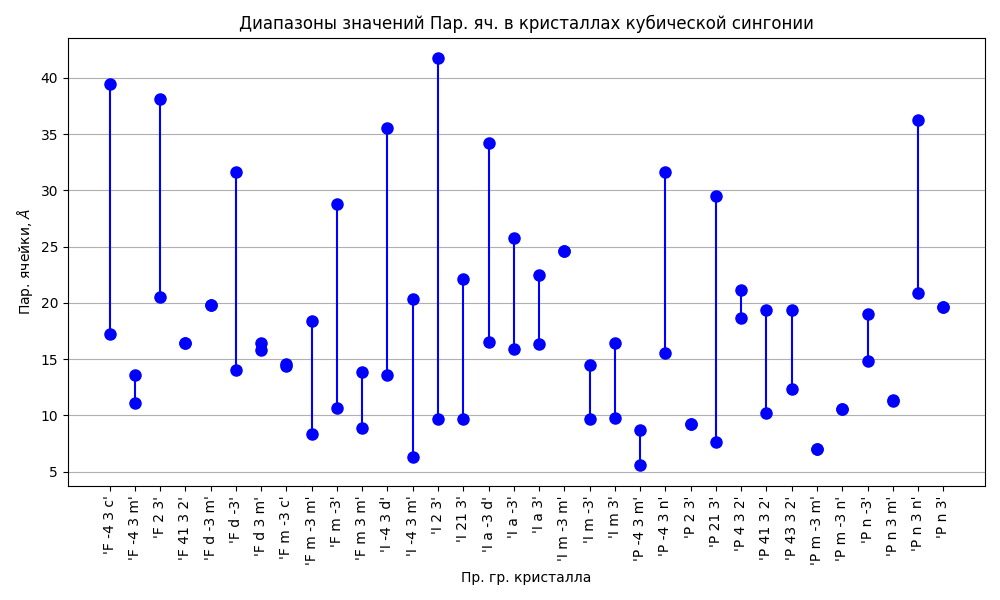
\includegraphics[scale=0.6]{plots_cell/cubic_syngony}
\caption{Диапазоны параметров ячейки для кристаллов кубической сингонии}
\end{figure}

\begin{table}[H]
\begin{tabular}{c|c|c|c|c}
Пр. гр. кристалла & Объем молекулы (\AA) & Пар. яч. (\AA) & $V_c$ & $V_f$\\
\hline
F 41 3 2 & 91.416 & 16.432 & 4210 & 1095\\
F m -3 c & 122.859 & 14.418 & 28830 & 7548\\
F m -3 c & 122.859 & 14.418 & 28830 & 7548\\
F m -3 & 42.148 & 10.610 & 19730 & 5132\\
F m -3 & 89.100 & 10.629 & 19730 & 5132\\
F m -3 & 84.495 & 10.867 & 19730 & 5132\\
F m -3 & 96.503 & 10.878 & 19730 & 5132\\
F m -3 & 136.278 & 10.644 & 19730 & 5132\\
I 2 3 & 1549.870 & 25.421 & 426 & 110\\
I 2 3 & 2477.170 & 41.766 & 426 & 110\\
I 2 3 & 188.394 & 18.849 & 426 & 110\\
I -4 3 d & 67.365 & 35.533 & 674 & 175\\
I -4 3 d & 60.574 & 31.150 & 674 & 175\\
I -4 3 d & 59.398 & 31.150 & 674 & 175\\
I a -3 d & 11.836 & 16.533 & 2175 & 569\\
I a -3 d & 11.930 & 16.536 & 2175 & 569\\
I m -3 m & 11.355 & 24.590 & 139651 & 36183\\
P 21 3 & 1816.530 & 21.023 & 172 & 46\\
P 21 3 & 2476.490 & 29.534 & 172 & 46\\
P 21 3 & 2432.170 & 29.534 & 172 & 46\\
P 21 3 & 128.696 & 19.380 & 172 & 46\\
P 21 3 & 129.574 & 19.381 & 172 & 46\\
P 21 3 & 1189.420 & 20.029 & 172 & 46\\
P 21 3 & 102.260 & 19.551 & 172 & 46\\
P 21 3 & 105.636 & 12.817 & 172 & 46\\
P 21 3 & 10.963 & 15.069 & 172 & 46\\
P 21 3 & 44.947 & 17.863 & 172 & 46\\
P 43 3 2 & 31.297 & 17.827 & 681 & 176\\
P -4 3 n & 38.114 & 20.028 & 469 & 121\\
P m -3 n & 177.878 & 10.520 & 15250 & 3952\\
P n 3 n & 1277.650 & 36.238 & 1363 & 352

\end{tabular}
\caption{Значения запрещенного объема для кристаллов с ассиметричными молекулами}
\end{table}

\nocite{*}
\pretolerance=3000 % предотвращает выход за пределы страницы
\printbibliography[title={\centering Литература}, heading=bibintoc]
\end{document}


    
